\section{Common Manuscript Mistakes}

Manuscript follows a strict set of rules and conventions, however there are a \emph{lot} of them and as such it's perfectly natural that children struggle to remember them all, resulting in mistakes.

Since there's not a huge amount of point attempting to build a system to recognise something it will never come across,I needed to establish exactly which mistakes were actually likely to occur, for which I referred to two main sources.

The first is Music Theory in Practice, \parencite{taylor2008music} which was mentioned in \cref{sec:music-book-taylor2008}. It's a book specifically written to teach music theory and has some great examples of mistakes a student should avoid.

My second source was real professional musicians and tutors but this involved a more hands on collection method which is covered in \cref{sec:teacher-data-gathering}.

\subsection{Gathering Professional Feedback}
\label{sec:teacher-data-gathering}

In order to build an application which can help to compensate for the absence of a tutor, we need to ensure that it can spot as many of the same mistakes as a tutor would.

The most logical way to establish precisely what these mistakes are is (surprise surprise) to ask the tutors, however when I did this, several of them found it difficult to express the mistakes they had seen children make without a piece of music in front of them.

I therefore devised the following method for gathering mistake data:

\begin{enumerate}
  \item Build the input section of the application such that a student can `free-draw' on a blank music staff.
  \item Set the student challenges and ask them to have a go at as many as they can
  \item Print out the attempts (labelled) and get a music tutor to mark them freehand
  \item Collate and summarise the feedback
\end{enumerate}

To save time (and paper) the marking was done 3-UP on a portrait sheet of A4, an example of one of the tutor feedback sheets can be seen in \cref{fig:teacher-sheet}. It should be noted that in some of the feedback tutors refer to errors differently, for example by using `the stem is on the wrong side' to mean that either a note stem is up when it should be down or that it's on the right when it should be on the left.

Evaluation of my application against this data is outlined in \todo[inline]{REFERENCE: where?} but for now I will just show specific examples which represent particular mistakes.

\begin{figure}[H]
  \centering
  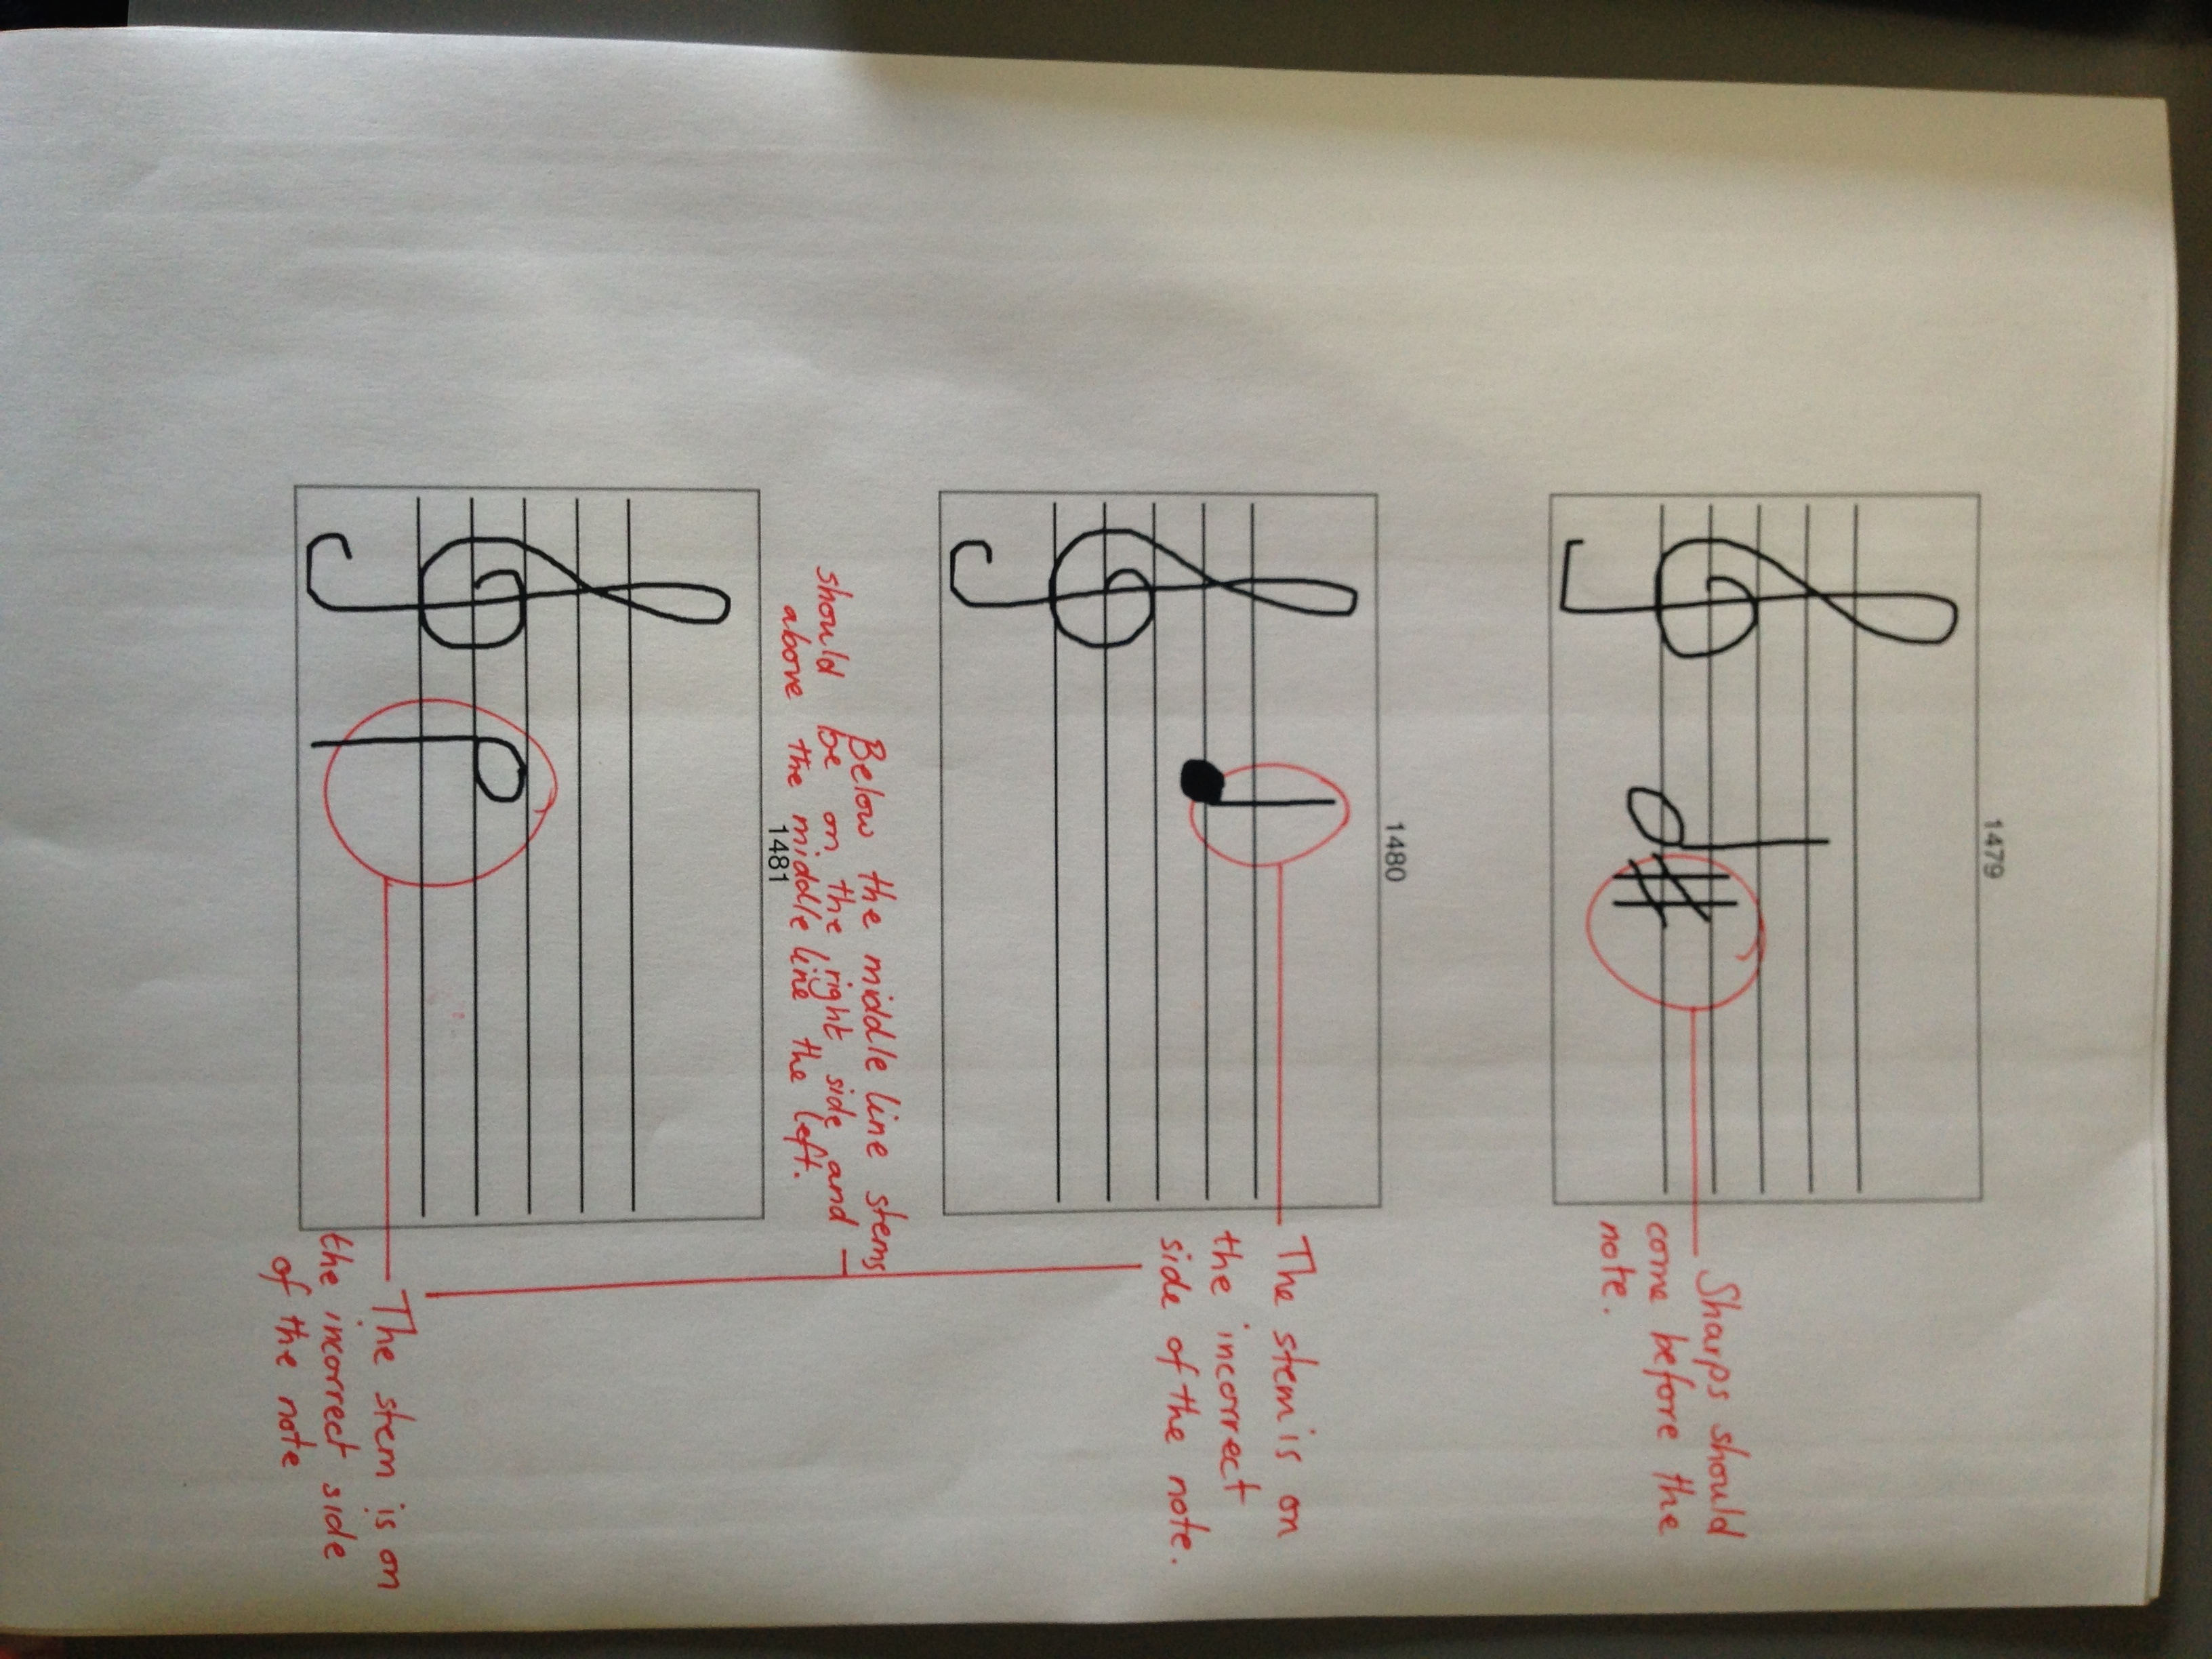
\includegraphics[width=\linewidth]{gfx/photos/teacher-sheet-1.jpg}
  \caption{Example of tutor-annotated manuscript}
  \label{fig:teacher-sheet}
\end{figure}

Once this data was collected I had a sample of \todo[inline]{COUNT HOW MANY STUDENT SAMPLES I HAD} marked samples \todo[inline,color=blue]{Put this full dataset at the end?} and I was able to extract some of the recurring issues which I've summarised in \cref{table:teacher-feedback-summary}. I present what is by no means an exhaustive list below and later on in \cref{sec:scoring} I go over how I actually identify, score and provide feedback to the student for a number of these mistakes.

\begin{table}[H]
    \renewcommand{\arraystretch}{1.8}
    \centering
    \begin{tabularx}{\textwidth}{ llll }
        \toprule

        Element & Issue & Description & Analysis \\
        \midrule
        Note Head       & Scale                  & \cref{sec:tf-note-head-size}              & \\
        Note Head       & Broken Lines           & \cref{sec:tf-note-head-broken}            & \\
        Note Head       & Angled                 & \cref{sec:tf-note-head-angled}            & \\
        Note Head       & Messy                  & \cref{sec:tf-note-head-messy}             & \\
        Stem            & Length                 & \cref{sec:tf-stem-length}                 & \\
        Stem            & Straightness           & \cref{sec:tf-stem-straightness}           & \\
        Stem            & Direction              & \cref{sec:tf-stem-direction}              & \\
        Stem            & Side                   & \cref{sec:tf-stem-side}                   & \\
        Stem            & Angle                  & \cref{sec:tf-stem-angle}                  & \\
        Quaver Tail     & Side                   & \cref{sec:tf-quaver-tail-side}            & \\
        Treble Clef     & Position               & \cref{sec:tf-treble-clef-location}        & \\
        Bass Clef       & Position               & \cref{sec:tf-bass-clef-location}          & \\
        Bass Clef       & Direction              & \cref{sec:tf-bass-clef-direction}         & \\
        Minim Rest      & Position               & \cref{sec:tf-minim-rest}                  & \\
        Sharp           & Ambiguous Position     & \cref{sec:tf-sharp-ambiguous}             & \\
        Key Signature   & Mixed Accidentals      & \cref{sec:tf-keysig-mixed}                & \\
        Key Signature   & Incorrect Octave       & \cref{sec:tf-keysig-octave}               & \\
        Key Signature   & Incorrect Ordering     & \cref{sec:tf-keysig-order}                & \\
        Key Signature   & Incorrect Accidentals  & \cref{sec:tf-keysig-incorrect}            & \\
        Beats \& Timing & Too Many Beats         & \cref{sec:tf-beats-too-many}              & \\
        Beats \& Timing & Too Few Beats          & \cref{sec:tf-beats-too-few}               & \\
        Beats \& Timing & Wrong Time Signature   & \cref{sec:tf-beats-wrong-time-signature}  & \\

        \bottomrule
    \end{tabularx}
    \caption{A brief summary of some mistakes which emerged from the preliminary data gathering. `FUTURE' indicates that analysis for the mistake hasn't yet been incorporated into the application}
    \label{table:note-lengths}
\end{table}


\subsection{Note Heads}
\subsubsection{Note Head Size}\label{sec:tf-note-head-size}
\todo[inline,color=red]{Manuscript Mistakes - Note Head Size, outside lines, space}

\subsubsection{Broken Note Heads}\label{sec:tf-note-head-broken}
\todo[inline,color=red]{Manuscript Mistakes - Broken Minims/Semibreves}

\subsubsection{Messy Note Heads}\label{sec:tf-note-head-messy}
\todo[inline,color=red]{Manuscript Mistakes - Messy Crotchet Heads}

\subsubsection{Angled Heads}\label{sec:tf-note-head-angled}
\todo[inline,color=red]{Manuscript Mistakes - Angled Semibreves}



\subsection{Note Stems}

\subsubsection{Stem Angle}\label{sec:tf-stem-angle}
\todo[inline,color=red]{Manuscript Mistakes - Stem Angle}

\subsubsection{Stem Straightness}\label{sec:tf-stem-straightness}
\todo[inline,color=red]{Manuscript Mistakes - Stem Wonky}

\subsubsection{Stem Direction}\label{sec:tf-stem-direction}
\todo[inline,color=red]{Manuscript Mistakes - Stem Direction}

\subsubsection{Stem Side}\label{sec:tf-stem-side}
\todo[inline,color=red]{Manuscript Mistakes - Stem Side}

\subsubsection{Stem Length}\label{sec:tf-stem-length}
\todo[inline,color=red]{Manuscript Mistakes - Stem Length}

\subsection{Quaver Tails}

\subsubsection{Quaver Tail Side}\label{sec:tf-quaver-tail-side}

\todo[inline,color=red]{Manuscript Mistakes - Quaver Tail Side}
\begin{figure}[H]
  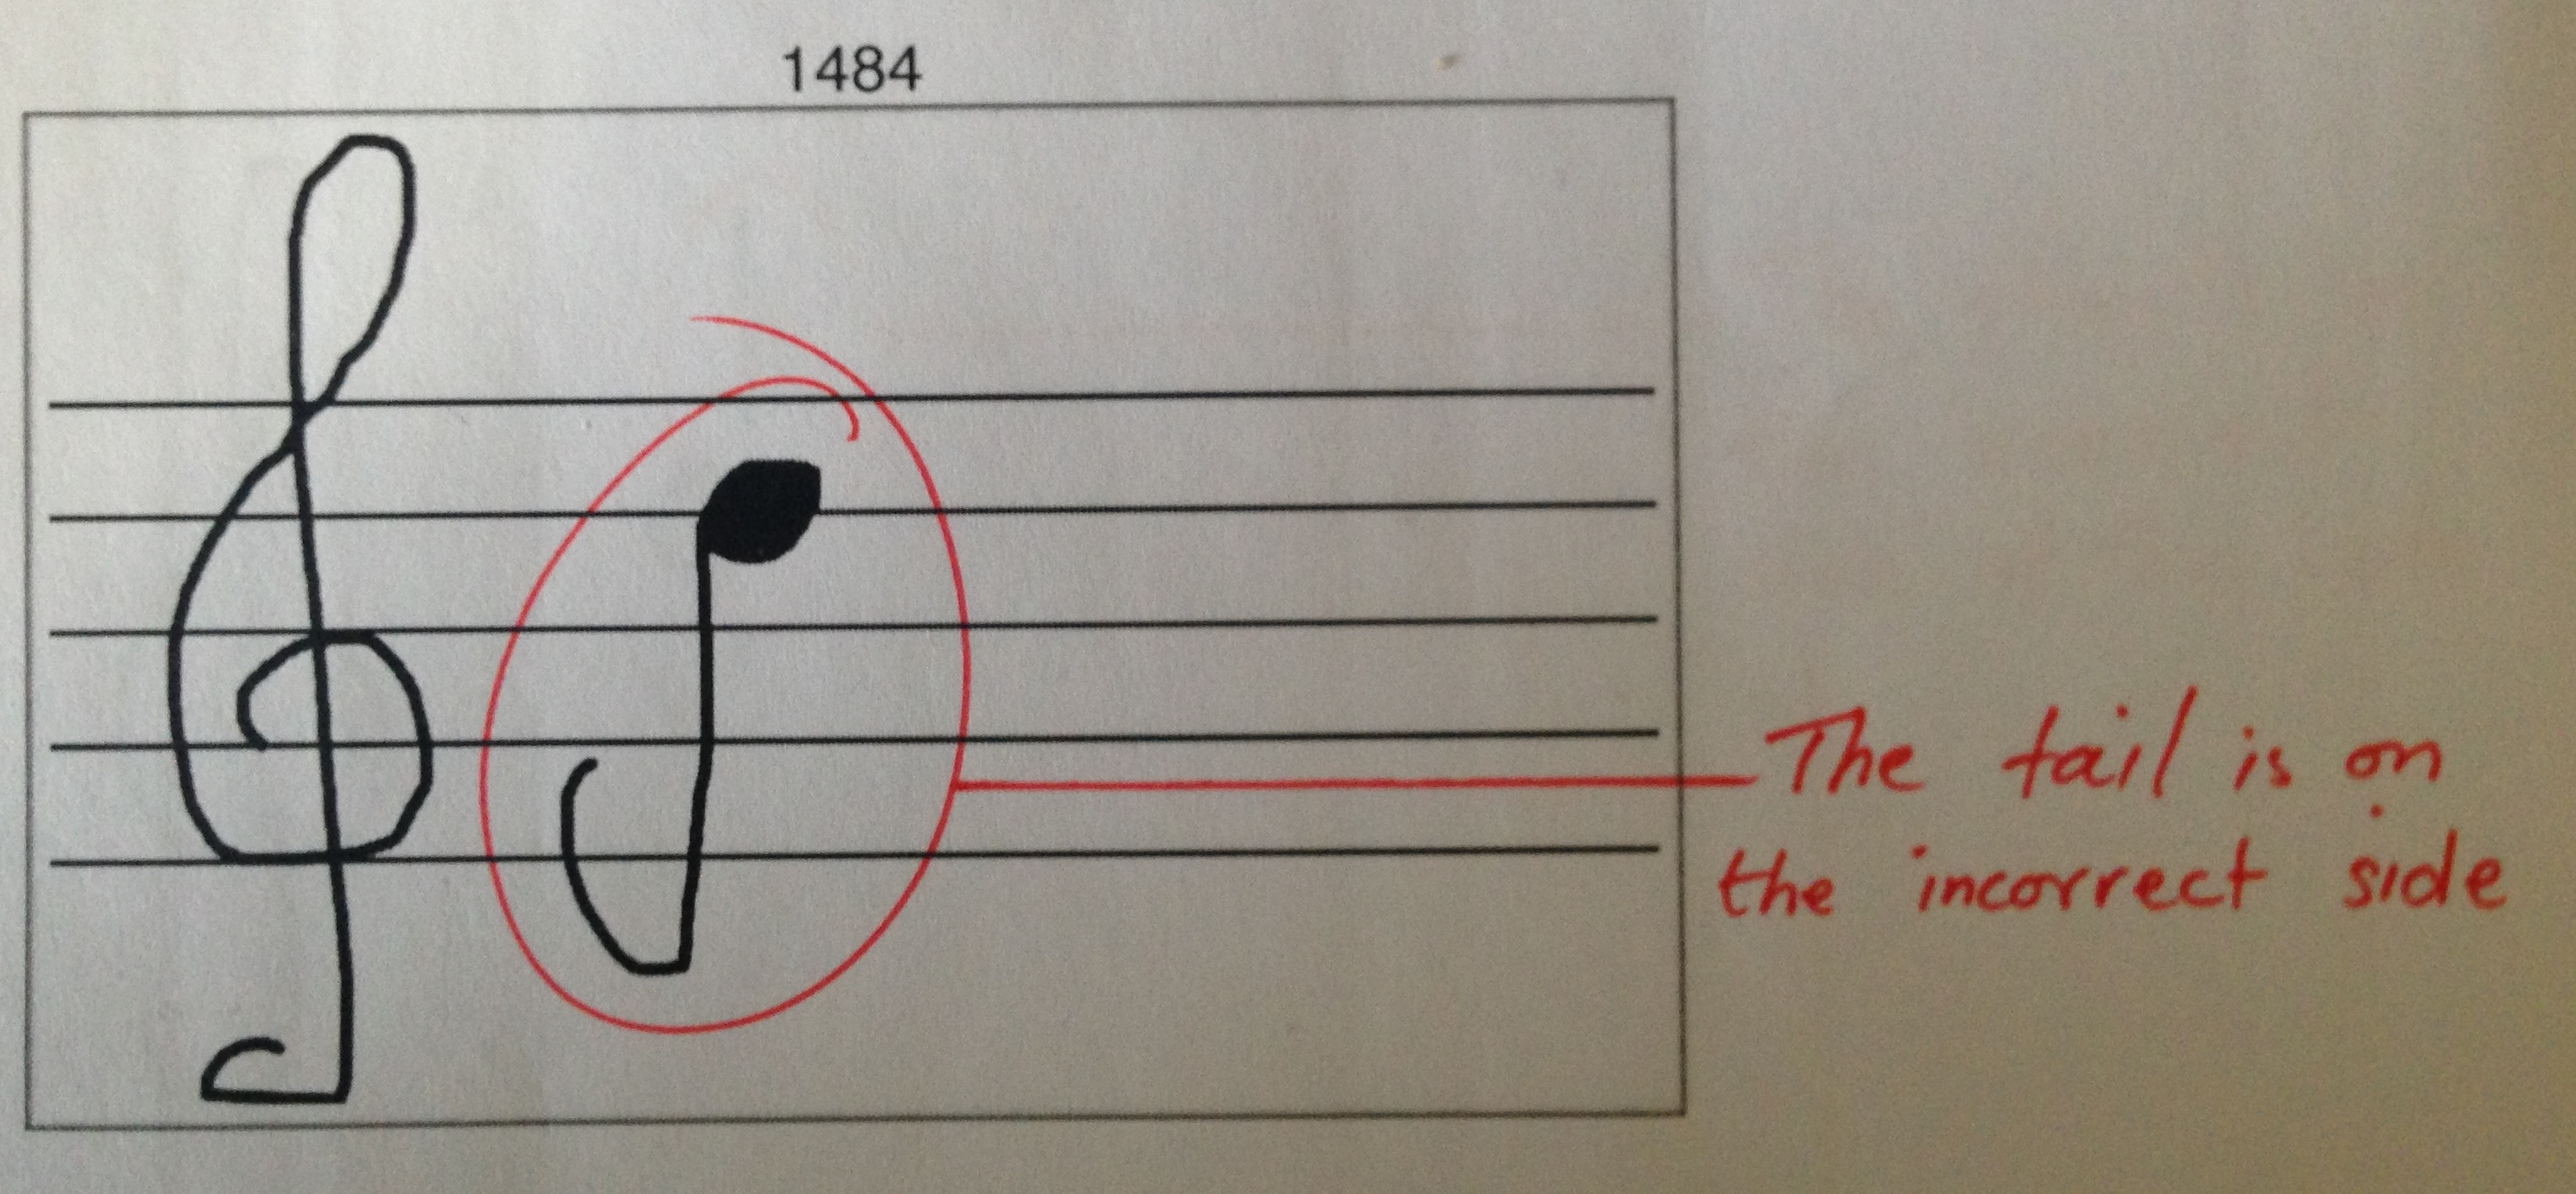
\includegraphics[width=\linewidth]{gfx/photos/teacher-bad-quavertail-side.jpg}
  \caption{Teacher's annotation of a bad quaver tail side}
  \label{fig:teacher-example-quaver-wrong-side}
\end{figure}

\subsection{Clefs}

\subsubsection{Treble Clef Location}\label{sec:tf-treble-clef-location}
\todo[inline,color=red]{Manuscript Mistakes - Treble Clef Location}

\subsubsection{Bass Clef Location}\label{sec:tf-bass-clef-location}
\todo[inline,color=red]{Manuscript Mistakes - Bass Clef Location}

\subsubsection{Bass Clef Direction}\label{sec:tf-bass-clef-direction}
\todo[inline,color=red]{Manuscript Mistakes - Bass Clef Horizontal Direction}

\subsection{Rests}

\subsubsection{Minim \& Semibreve Rests}\label{sec:tf-minim-rest}
\todo[inline,color=red]{Manuscript Mistakes - Minim/Semibreve Rest not in right place too high/low}

\subsection{Accidentals}
\subsubsection{Ambiguous Sharp Positions}\label{sec:tf-sharp-ambiguous}

\subsection{Key Signatures}
\subsubsection{Mixed Accidentals}\label{sec:tf-keysig-mixed}
\todo[inline,color=red]{Manuscript Mistakes - Mixed Accidentals}

\subsubsection{Swrong Octave}\label{sec:tf-keysig-octave}
\todo[inline,color=red]{Manuscript Mistakes - Wrong Octave}

\subsubsection{Incorrect Order}\label{sec:tf-keysig-order}
\todo[inline,color=red]{Manuscript Mistakes - Incorrect Order}

\subsubsection{Incorrect Pitch}\label{sec:tf-keysig-incorrect}
\todo[inline,color=red]{Manuscript Mistakes - Incorrect Accidentals}

\subsection{Beats and Timing}

\subsubsection{Too Many Beats}\label{sec:tf-beats-too-many}
\todo[inline,color=red]{Manuscript Mistakes - Too many beats in a bar}

\subsubsection{Too Few Beats}\label{sec:tf-beats-too-few}
\todo[inline,color=red]{Manuscript Mistakes - Too few beats in a bar}

\subsubsection{Wrong Time Signature}\label{sec:tf-beats-wrong-time-signature}
\todo[inline,color=red]{Manuscript Mistakes - Wrong time signature?}




